\documentclass[12pt,letterpaper]{article}
\usepackage[utf8]{inputenc}
\usepackage[spanish]{babel}
\usepackage{graphicx}
\usepackage[left=2cm,right=2cm,top=2cm,bottom=2cm]{geometry}
\usepackage{graphicx} % figuras
% \usepackage{subfigure} % subfiguras
\usepackage{float} % para usar [H]
\usepackage{amsmath}
%\usepackage{txfonts}
\usepackage{stackrel} 
\usepackage{multirow}
\usepackage{enumerate} % enumerados
\renewcommand{\labelitemi}{$-$}
\renewcommand{\labelitemii}{$\cdot$}
% \author{}
% \title{Caratula}
\begin{document}

% Fancy Header and Footer
% \usepackage{fancyhdr}
% \pagestyle{fancy}
% \cfoot{}
% \rfoot{\thepage}
%

% \usepackage[hidelinks]{hyperref} % CREA HYPERVINCULOS EN INDICE

% \author{}
\title{Caratula}

\begin{titlepage}
\begin{center}
\large{UNERSIDAD PRIVADA DE TACNA}\\
\vspace*{-0.025in}
\begin{figure}[htb]
\begin{center}

\includegraphics[width=8cm]{./Imagenes/logo}
\end{center}
\end{figure}
\vspace*{0.15in}
INGENIERIA DE SISTEMAS  \\

\vspace*{0.5in}
\begin{large}
TITULO:\\
\end{large}

\vspace*{0.1in}
\begin{Large}
\textbf{INFORME DE LABORATORIO No 03} \\
\end{Large}

\vspace*{0.3in}
\begin{Large}
\textbf{CURSO:} \\
\end{Large}

\vspace*{0.1in}
\begin{large}
INTELIGENCIA DE NEGOCIOS\\
\end{large}

\vspace*{0.3in}
\begin{Large}
\textbf{DOCENTE(ING):} \\
\end{Large}

\vspace*{0.1in}
\begin{large}
 Patrick Cuadros Quiroga\\
\end{large}

\vspace*{0.2in}
\vspace*{0.1in}
\begin{large}
Alumno: \\
\begin{flushleft}
Quispe Mamani , Angelo Brian		\hfill	(2015052719) \\
\end{flushleft}
\end{large}
\end{center}

\end{titlepage}


\tableofcontents % INDICE
\thispagestyle{empty} % INDICE SIN NUMERO
\newpage
\setcounter{page}{1} % REINICIAR CONTADOR DE PAGINAS DESPUES DEL INDICE

 \section{Actividad No 01 – DESARROLLO} 
Conectando Power BI \\
	
	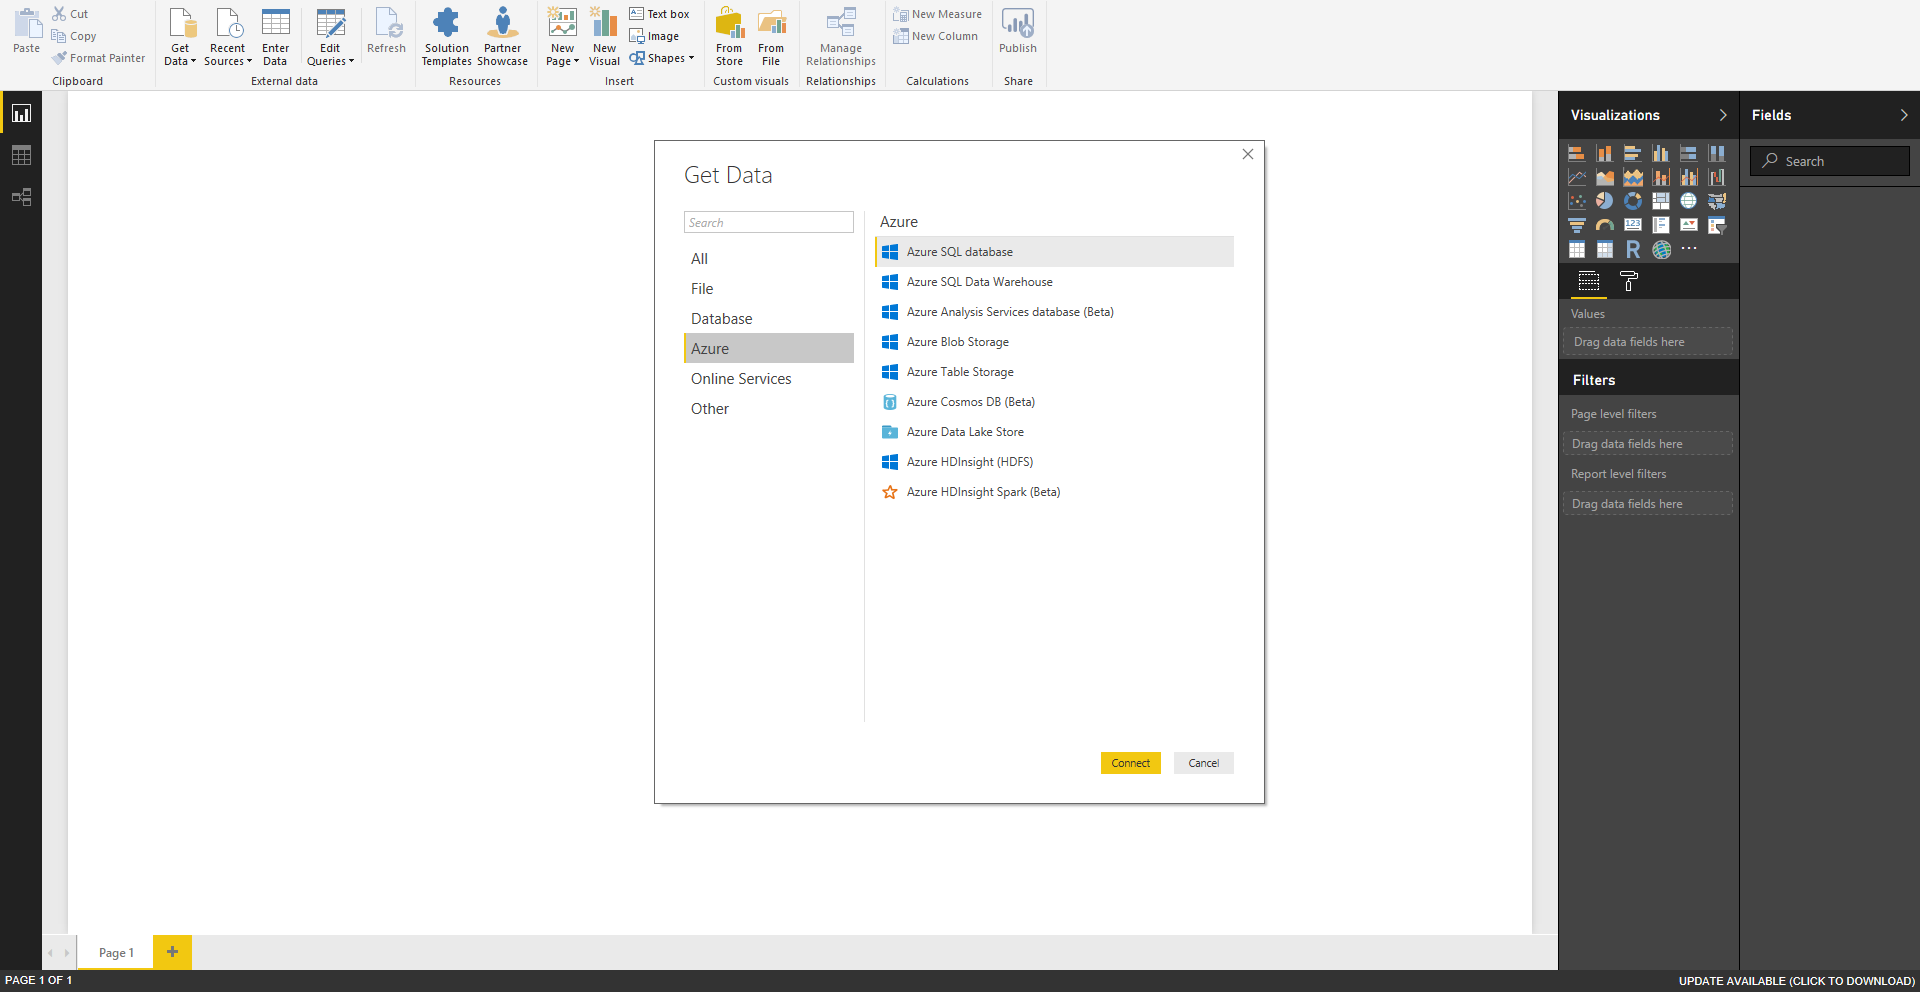
\includegraphics[width=15cm]{./Imagenes/11.png} 

	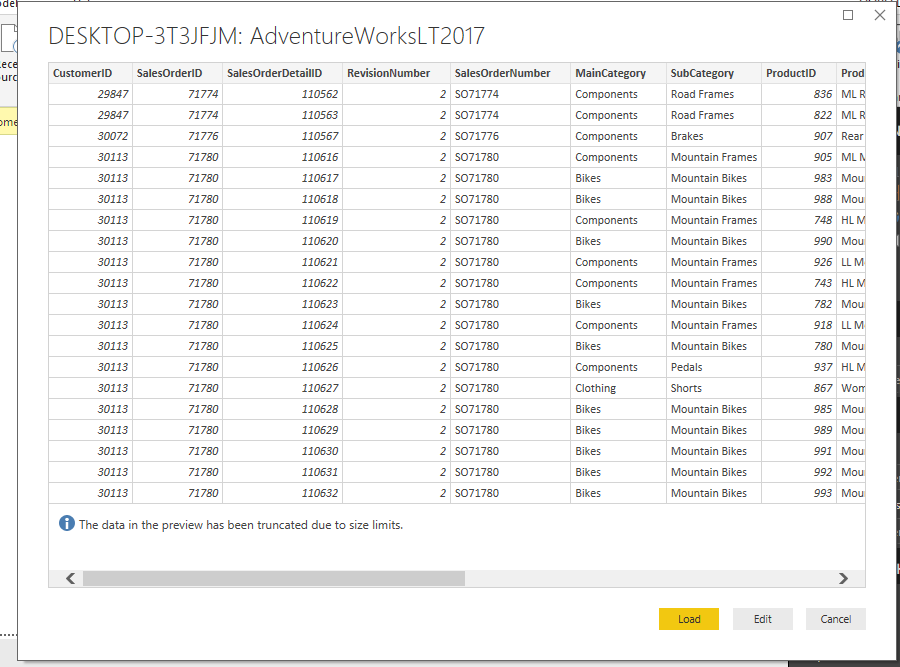
\includegraphics[width=15cm]{./Imagenes/12.png}

	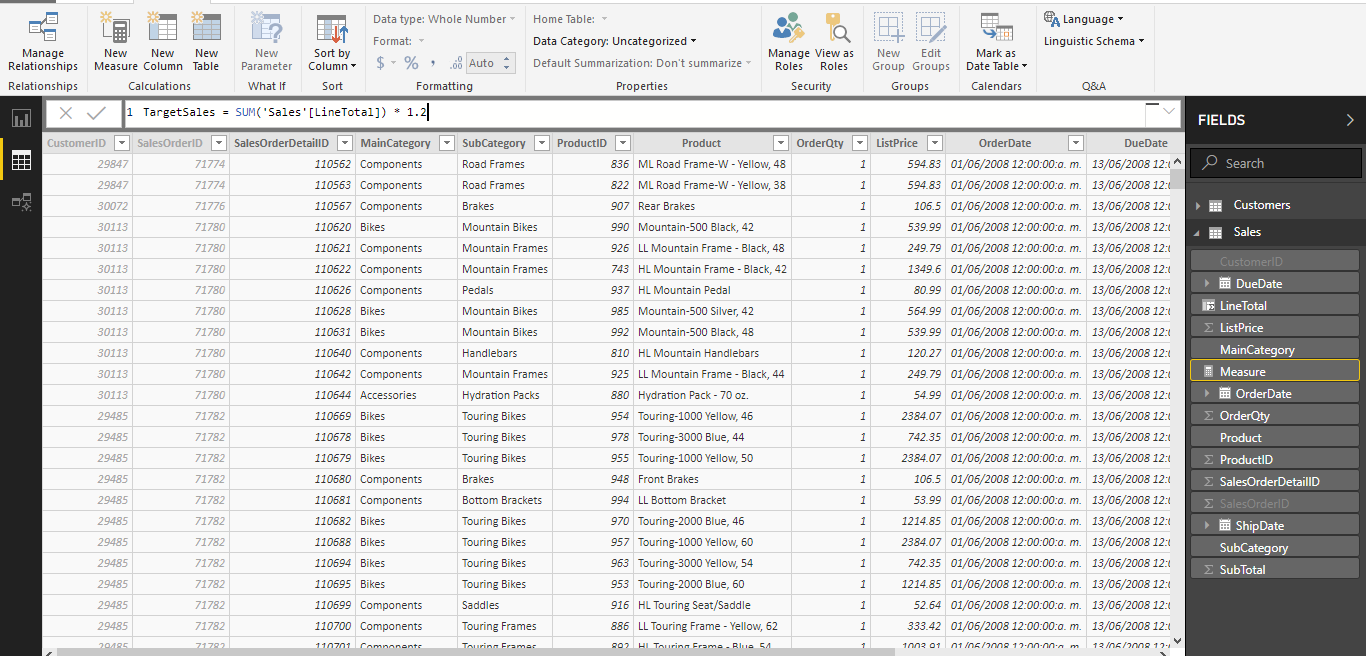
\includegraphics[width=15cm]{./Imagenes/13.png}

	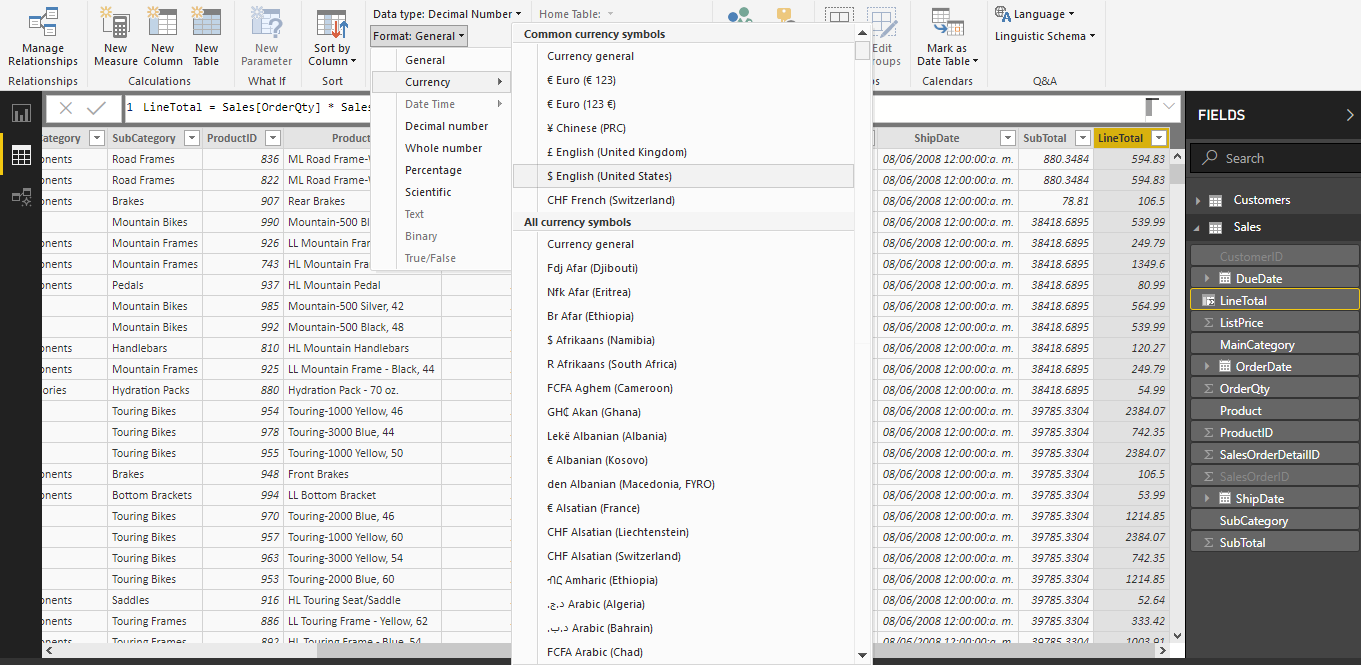
\includegraphics[width=15cm]{./Imagenes/14.png}

	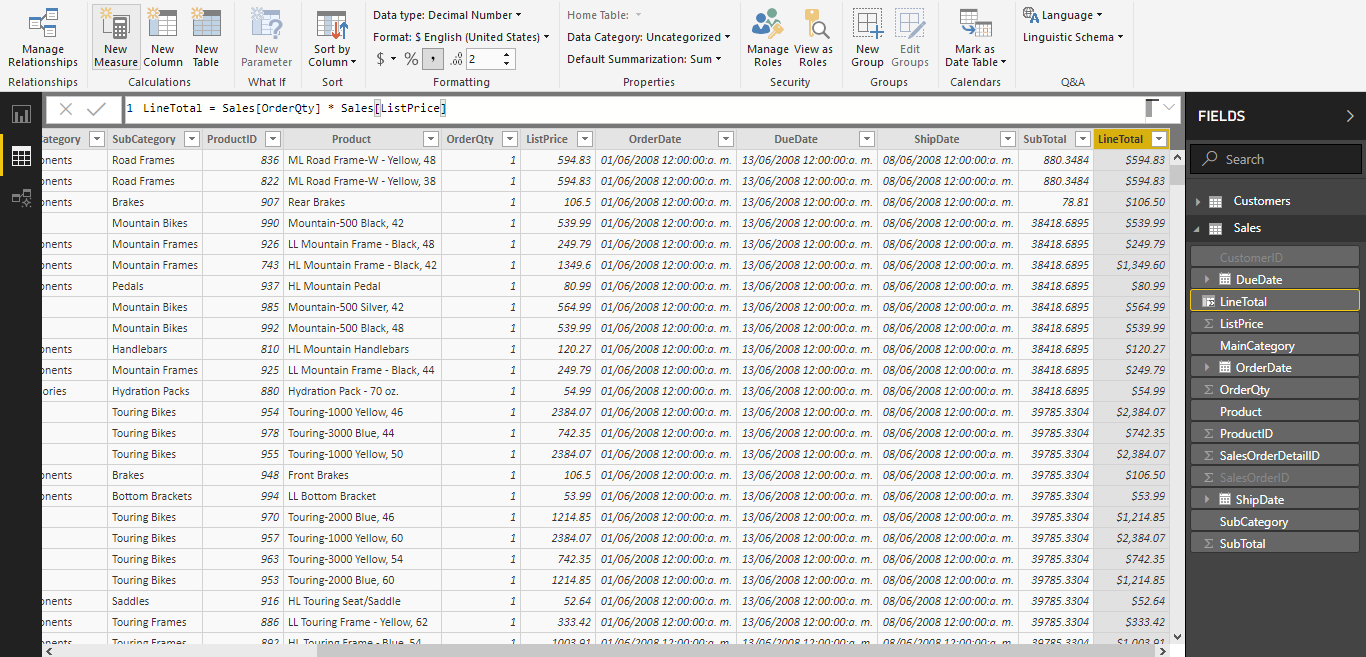
\includegraphics[width=15cm]{./Imagenes/15.png}

	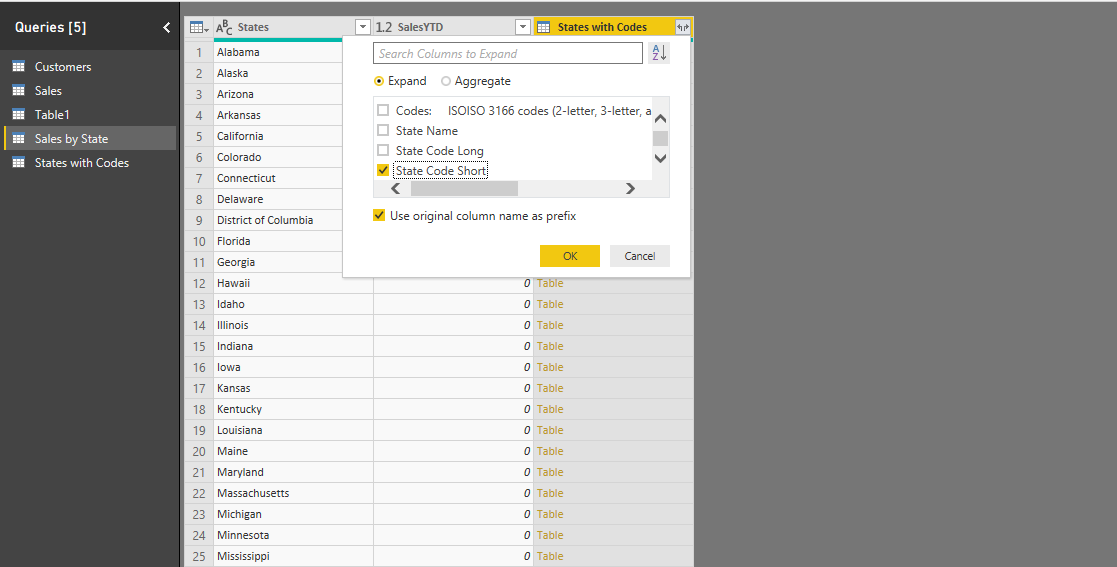
\includegraphics[width=15cm]{./Imagenes/16.png}

	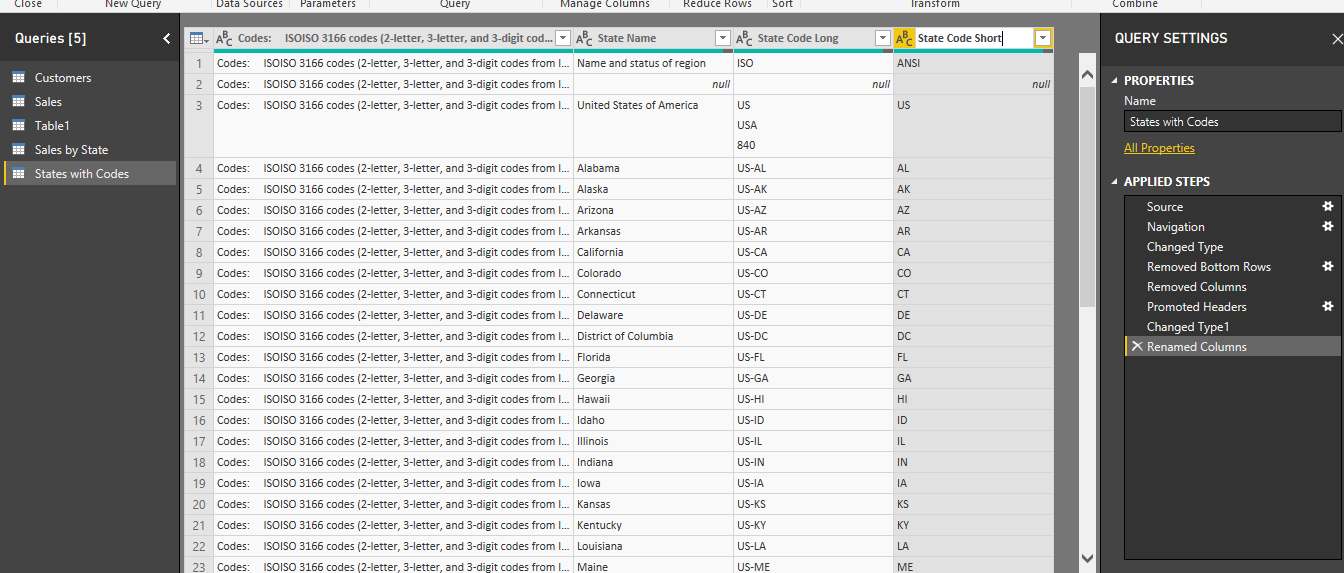
\includegraphics[width=15cm]{./Imagenes/17.png}

	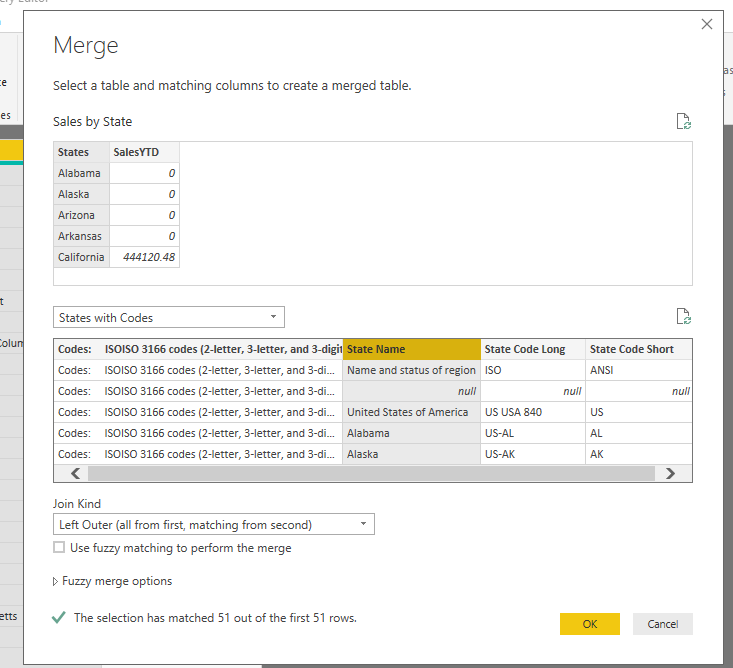
\includegraphics[width=15cm]{./Imagenes/18.png}
	




	



\section{Actividad No 01 – DESARROLLO} 

 Shape Data \\

	\begin{center}
	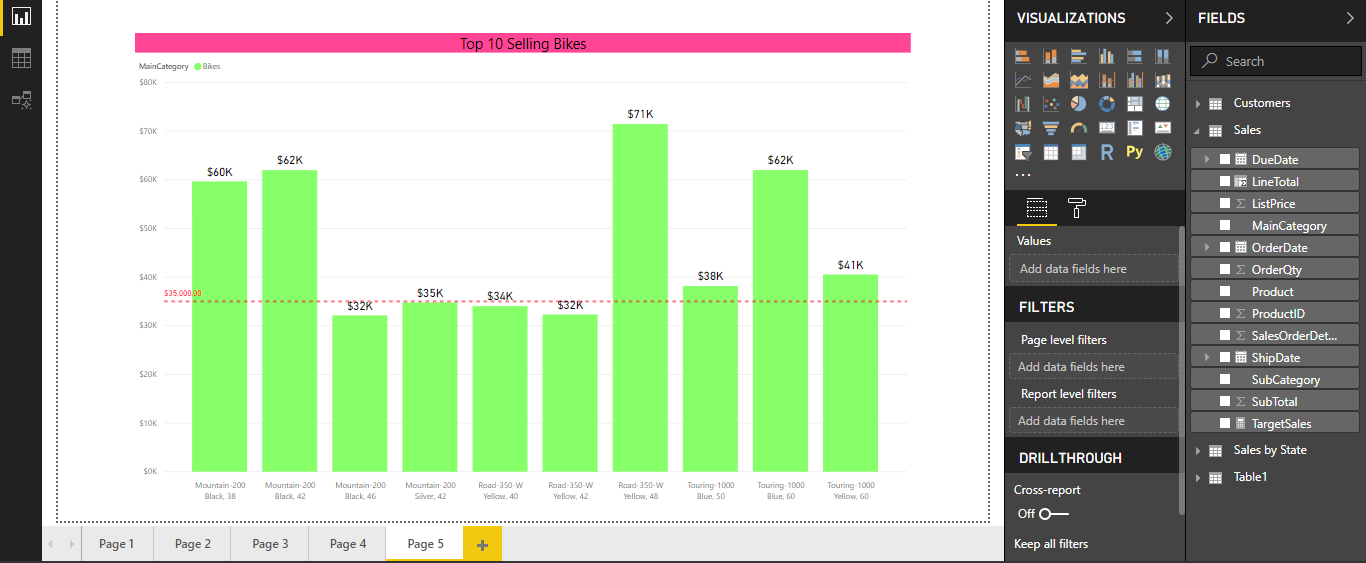
\includegraphics[width=15cm]{./Imagenes/21.png}
	\end{center}	
	\begin{center}
	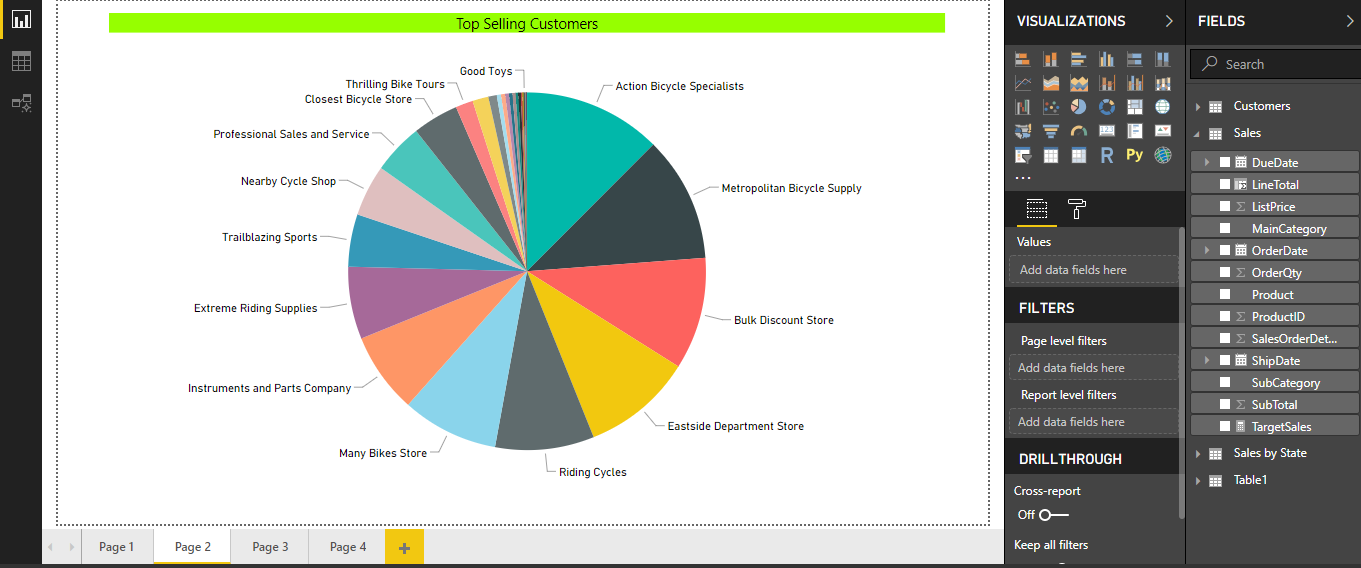
\includegraphics[width=15cm]{./Imagenes/22.png}
	\end{center}	
\begin{center}
	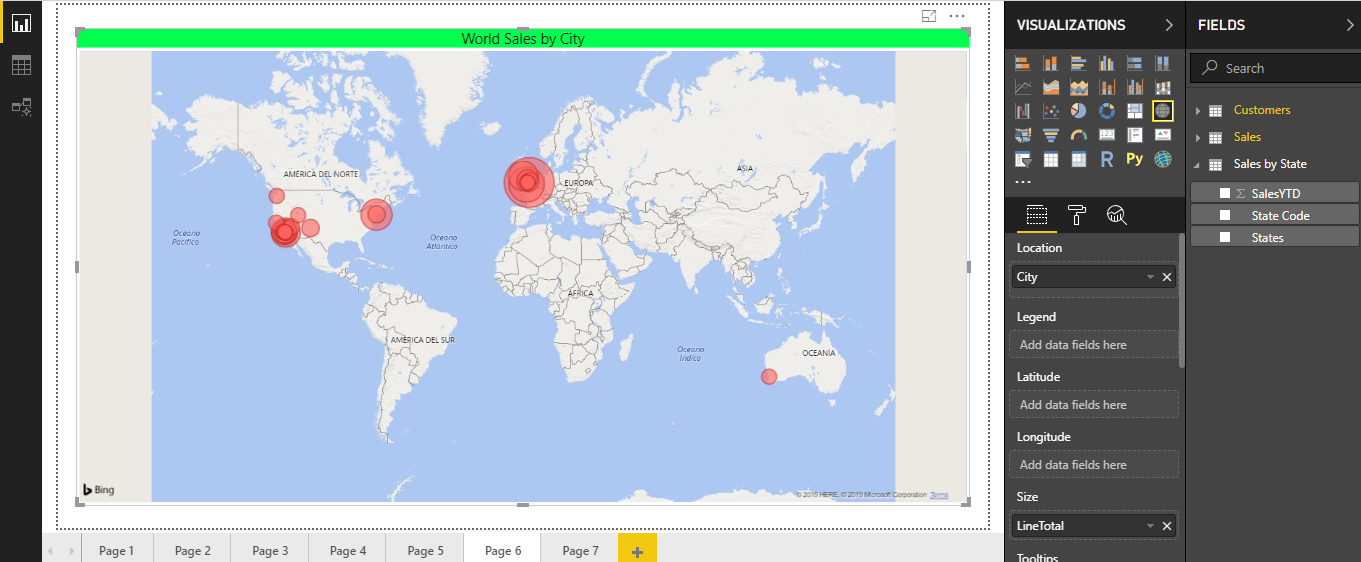
\includegraphics[width=15cm]{./Imagenes/23.png}
	\end{center}	
\begin{center}
	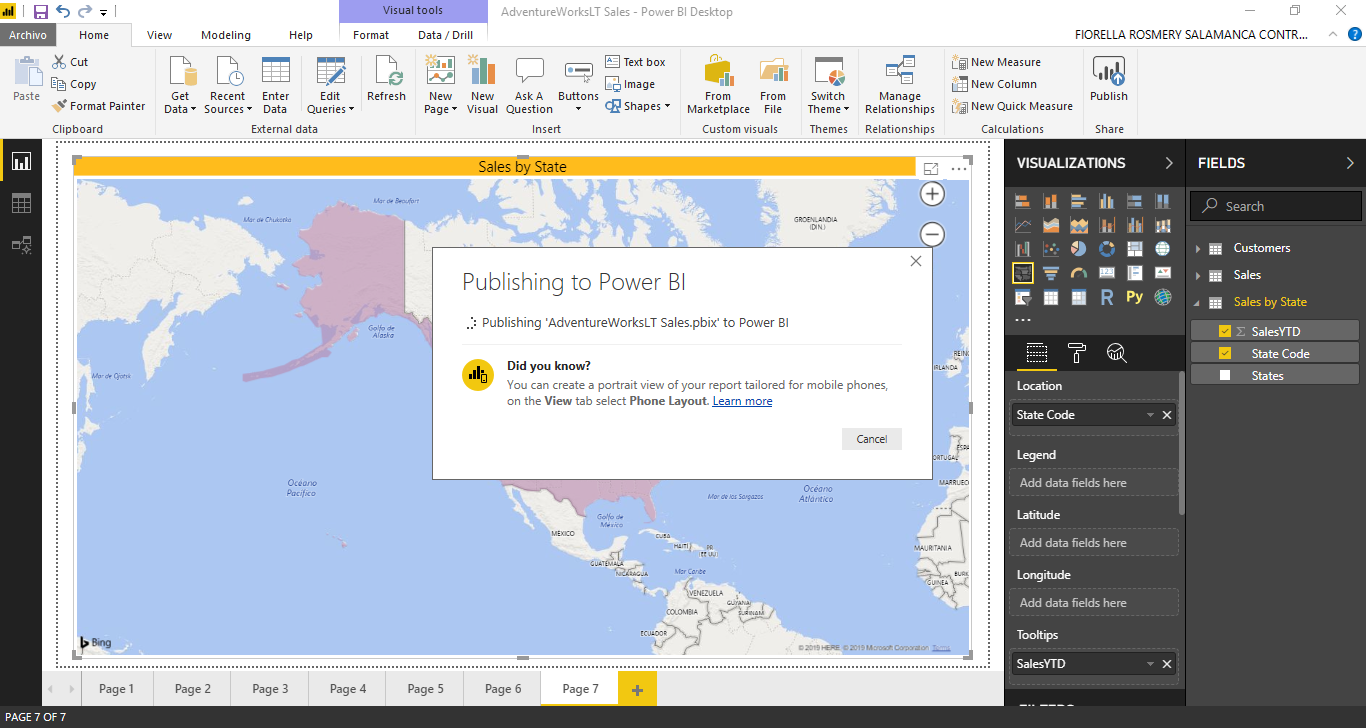
\includegraphics[width=15cm]{./Imagenes/24.png}
	\end{center}	
\begin{center}
	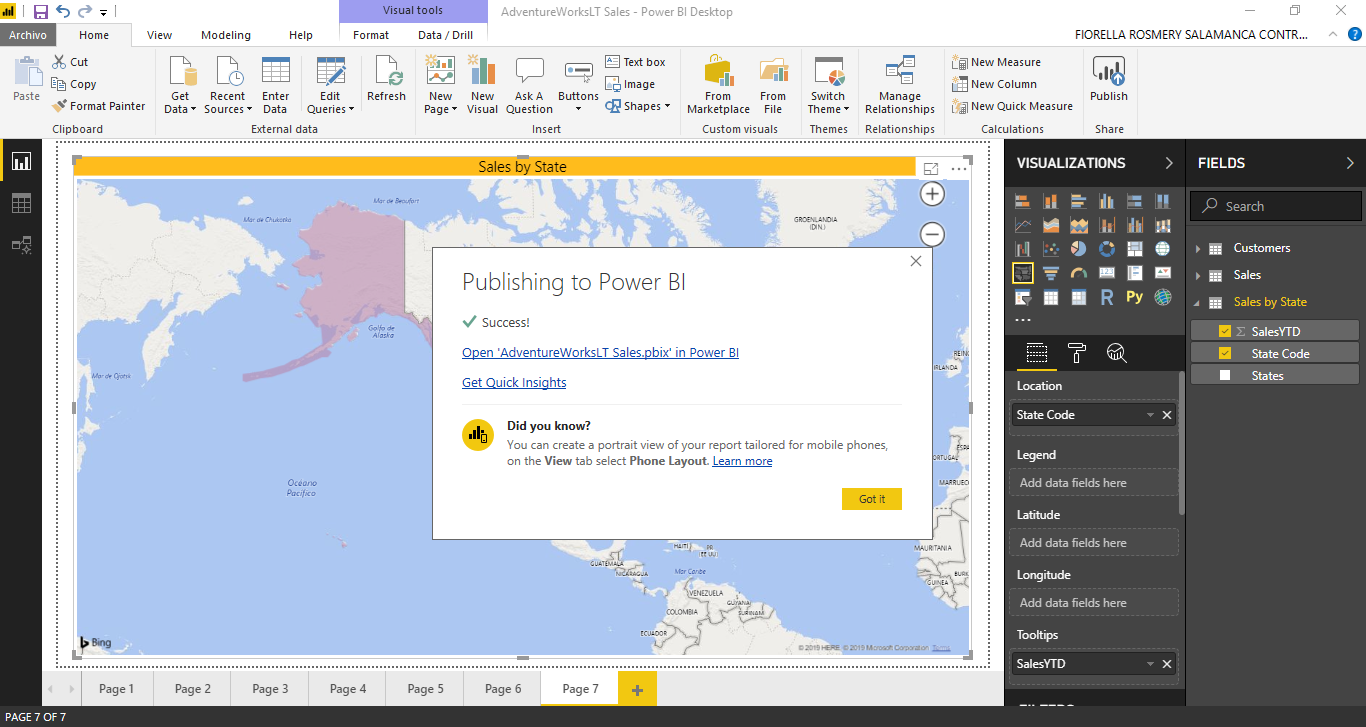
\includegraphics[width=15cm]{./Imagenes/25.png}
	\end{center}	
\section{Actividad No 01 – DESARROLLO} 

         Combine Data \\

	\begin{center}
	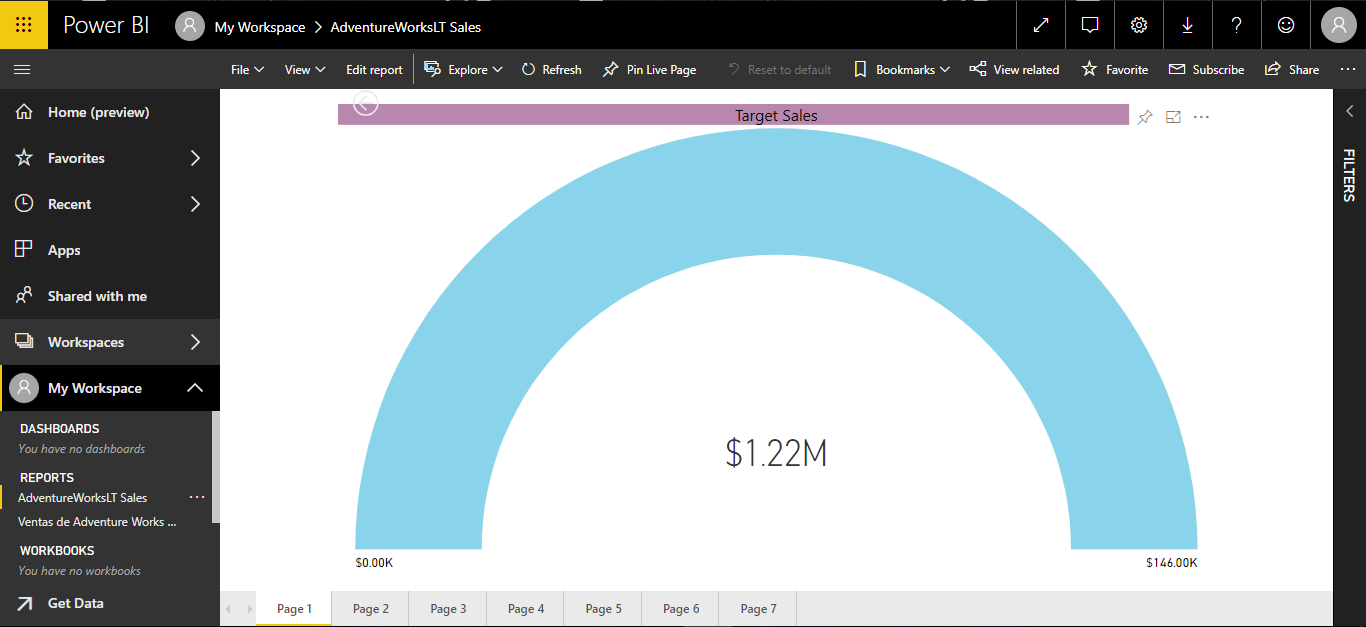
\includegraphics[width=15cm]{./Imagenes/31.png}
	\end{center}	
\begin{center}
	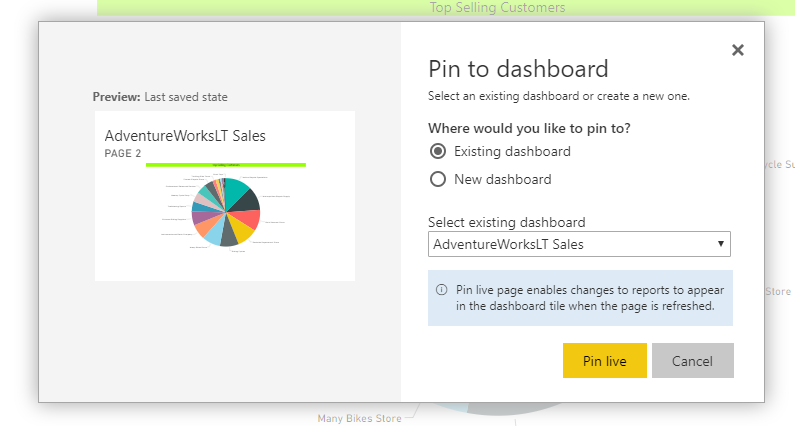
\includegraphics[width=15cm]{./Imagenes/32.png}
	\end{center}	

	
\begin{center}
	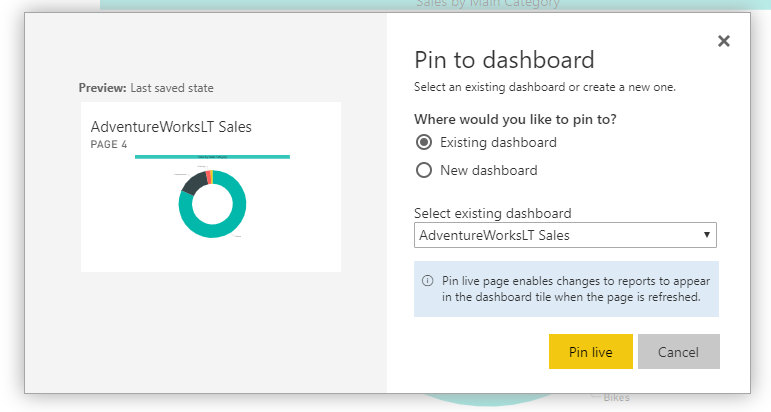
\includegraphics[width=15cm]{./Imagenes/33.png}
	\end{center}	

	

	

\end{document}
